\documentclass[tikz]{standalone}

\usepackage{amsmath}
\usepackage{unicode-math}
\usepackage{mathtools}
\usepackage{derivative}

\setmainfont{Stix Two Text}
\setmathfont{Stix Two Math}

\usetikzlibrary{arrows.meta,fit,positioning}

\renewcommand{\familydefault}{\sfdefault}

% prefix equation numbers with section number
\numberwithin{equation}{section}

\DeclarePairedDelimiter{\ceil}{\lceil}{\rceil}
\DeclarePairedDelimiter{\floor}{\lfloor}{\rfloor}
\DeclarePairedDelimiter{\abs}{\lvert}{\rvert}
\DeclarePairedDelimiter{\norm}{\lVert}{\rVert}
\DeclarePairedDelimiter{\bra}{\langle}{\rvert}
\DeclarePairedDelimiter{\ket}{\lvert}{\rangle}
\DeclarePairedDelimiter{\expval}{\langle}{\rangle}
\DeclarePairedDelimiter{\norder}{\mathcolon}{\mathcolon}
\DeclarePairedDelimiter{\anorder}{\typecolon}{\typecolon}
	
\newcommand{\laplace}{\mbfnabla^2}
\newcommand{\trans}{{\scriptscriptstyle\mathsf{T}}}

\newcommand{\vdot}{\cdot}
\newcommand{\vcross}{\vectimes}
\newcommand{\vb}[1]{\symbfup{#1}}
\newcommand{\vu}[1]{\hat{\vb{#1}}}
\newcommand*\dd[2][\relax]{\mathop{\ifx\relax#1\odif{#2}\else \odif[order={#1}]{#2}\fi\,}}

\newcommand{\vacuum}{\ket*{\vb{0}}}

\DeclareMathOperator{\trace}{Tr}
\DeclareMathOperator{\sinc}{sinc}

\AtBeginDocument{
	\let\Re\relax
	\let\Im\relax
	\DeclareMathOperator{\Re}{Re}
	\DeclareMathOperator{\Im}{Im}

	\renewcommand{\div}{\mathop{\mbfnabla\vdot}}
	\newcommand{\curl}{\mathop{\mbfnabla\vectimes}}
}

\DeclarePairedDelimiterX{\comm}[2]{[}{]}{#1,#2}

\DeclarePairedDelimiterX{\braket}[2]{\langle}{\rangle}{#1\delimsize\vert#2}
\DeclarePairedDelimiterX{\ketbra}[1]{\lvert}{\rvert}{#1\rangle\delimsize\langle#1}



\usetikzlibrary{arrows.meta,fit,positioning}

\begin{document}
	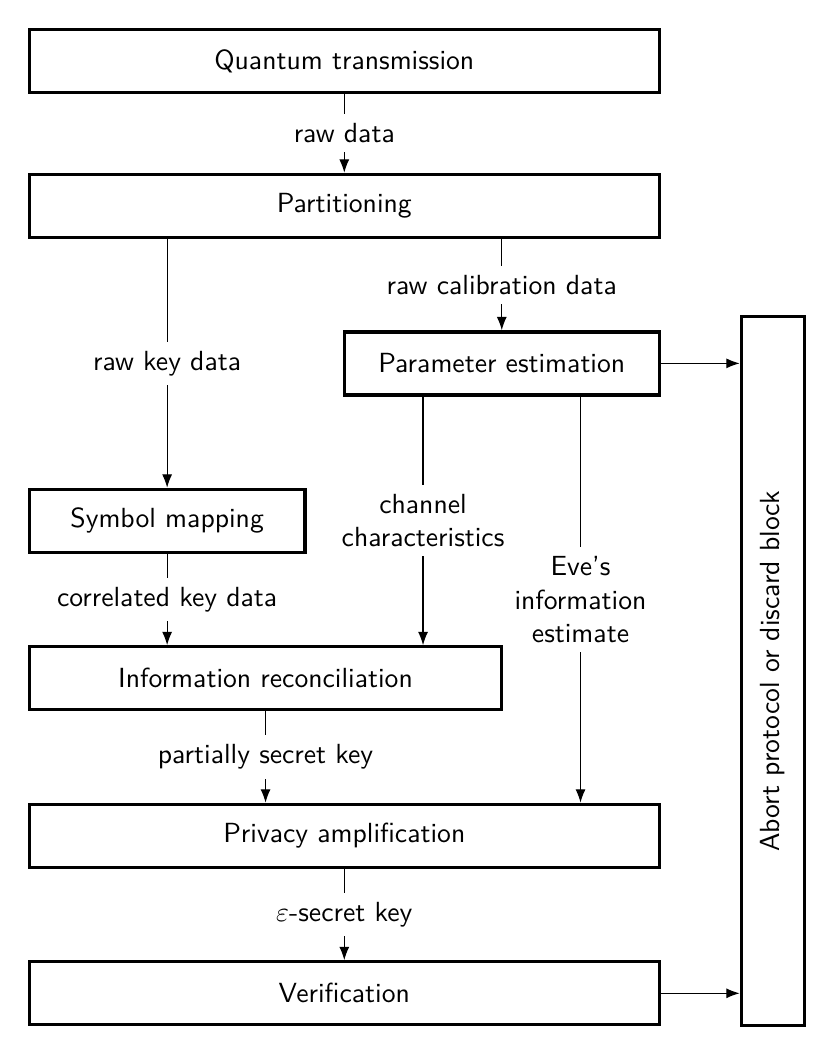
\begin{tikzpicture}[
		node distance=2cm,
		block/.style={draw, very thick, minimum height=0.8cm},
	]
		\node[block, minimum width=8cm] (qt) {Quantum transmission};
		\node[block, minimum width=8cm, below=1cm of qt] (pt) {Partitioning};		
		\node[block, below=of pt.east, anchor=east, minimum width=4cm] (pe) {Parameter estimation};
		\node[block, below=4cm of pt.west, anchor=west, minimum width=3.5cm] (sm) {Symbol mapping};
		\node[block, below=of sm.west, anchor=west, minimum width=6cm] (ir) {Information reconciliation};
		\node[block, below=of ir.west, anchor=west, minimum width=8cm] (pa) {Privacy amplification};
		\node[block, below=of pa.west, anchor=west, minimum width=8cm] (ver) {Verification};
		
		\draw[-Latex] (qt) -- (pt) node[midway, fill=white]{raw data};
		\draw[Latex-] (sm.north) -- (sm.north|-pt.south) node[midway, fill=white] {raw key data};
		\draw[Latex-] (pe.north) -- (pe.north|-pt.south) node[midway, fill=white] {raw calibration data};
		\draw[-Latex] (sm.south) -- (sm.south|-ir.north) node[midway, fill=white] {correlated key data};
		\draw[-Latex] (ir.south) -- (ir.south|-pa.north) node[midway, fill=white] {partially secret key};
		\draw[-Latex] (pa) -- (ver) node[midway, fill=white] {$\varepsilon$-secret key};
		\begin{scope}[transform canvas={xshift=-1cm}]
			\draw[-Latex] (pe.south) -- (pe.south|-ir.north) node[midway, fill=white, align=center]{channel\\characteristics};
		\end{scope}
		\begin{scope}[transform canvas={xshift=1cm}]
			\draw[-Latex] (pe.south) -- (pe.south|-pa.north) node[midway, fill=white, align=center]{Eve's\\information\\estimate};
		\end{scope}
		
		\node[block, right=1cm of qt, rotate=90, anchor=north, xshift=-7.75cm, minimum width=9cm] (abort) {Abort protocol or discard block};
		\draw[-Latex] (pe.east) -- (pe.east-|abort.north);
		\draw[-Latex] (ver.east) -- (ver.east-|abort.north);
	\end{tikzpicture}
\end{document}